\documentclass[12pt,a4paper]{article}
\usepackage[UTF8]{ctex}
\usepackage[backend=biber]{biblatex}
\DefineBibliographyStrings{english}{%
  references = {参考文献},
}
\addbibresource{report.bib}
\usepackage{amsmath,amsthm,amssymb,graphicx,multirow,float,caption,siunitx}
\usepackage{geometry}
\geometry{left=2.54cm, right=2.54cm, top=3.18cm, bottom=3.18cm}
\usepackage{enumitem}
\usepackage{subcaption,booktabs,diagbox}
\setenumerate[1]{itemsep=0pt,partopsep=0pt,parsep=\parskip,topsep=5pt}
\setitemize[1]{itemsep=0pt,partopsep=0pt,parsep=\parskip,topsep=5pt}
\setdescription{itemsep=0pt,partopsep=0pt,parsep=\parskip,topsep=5pt}
\usepackage{adjustbox}
\usepackage[graphicx]{realboxes}
\usepackage{rotating}

\usepackage{titlesec}

\newcommand{\be}[1]{
    \begin{equation}
        #1
    \end{equation}
}

\newcommand{\bfig}[3]{
    \begin{figure}[H]
        \centering
        \includegraphics[width=#1\textwidth]{#2}
        \caption{#3}
    \end{figure}
}

\titleformat{\section}%设置section的样式
{\raggedright\large\bfseries}%右对齐,4号字,加粗
{\thesection .\quad}%标号后面有个点
{0pt}%sep label和title之间的水平距离
{}%标题前没有内容

\title{\vspace{-4cm}\Large 塞曼效应实验报告}  %文章标题
\author{\kaishu 学号:202111030007 \hspace{2cm} 姓名:郑晓旸}   %作者的名称
\date{}

\begin{document}
\maketitle

\begin{abstract}
本实验利用 F-P 腔观察了汞绿线和汞黄线的干涉谱线. 在不加外磁场的情况下, 成功观察到了汞黄线的双线结构. 
并且在外加磁场的条件下, 观察到了谱线的塞曼分裂, 分别为汞绿线反常塞曼
效应和汞黄线正常塞曼效应. 其中汞绿线分裂为9条谱线, 汞黄线分裂为3条谱线. 
实验中定性观察了汞绿线和汞黄线, 并且分析了谱线的偏振特性. 得到的结论是, 汞绿线的塞曼效应中有6条$\sigma$线, 3条
$\pi$线, 汞黄线的塞曼效应中有2条$\sigma$线, 1条
$\pi$线. 利用塞曼效应的分裂间距测量了磁场大小, 并与电流标定结果比较。其中塞曼分裂测量磁场与电
流标定磁场误差在 5\%左右, 并进行了可能的误差分析. 


\bf{关键词: 塞曼效应\quad 法布里珀罗干涉仪\quad 汞光谱}
\end{abstract}

\section{引言}

在历史上, 塞曼效应指引着人们在电子的量子力学方程中引入了自旋的概念, 揭示了原子中电子的角动量的分类, 及不同角动量发生耦合的原子结构信息. 

在实验中, 为了观察这样的精细谱线结构, 使用了法布里珀罗干涉仪. 其原理为多光束干涉, 主要用于精确测量和控制光的频率和波长, 被广泛应用在通信、激光和光谱学领域. 
当代工艺已经能够制造出非常精密且可调谐的法布里-佩罗干涉仪. \cite{lecturenote}

本实验将使用法布里珀罗干涉仪观察汞绿线(546.1nm)和汞黄线(579.0)的塞曼分裂效应, 并通过谱线的分裂间距推测原子结构和磁场的一些信息. 


\section{原理}
原子体系在引入外磁场后, 发生退简并效应, 每一个用总角动量J标记的能级劈裂为2J+1个能级, 这些能级用新的量子数M标记. 其中$M=-J,-J+1,...,J-1,J$. 
这些能级的能量, 可以利用劈裂前的能级$E_{0}$表示为: 
\begin{equation}
E=E_{0}+\Delta E=E_{0}+M g \mu_{B} B
\end{equation}

其中$\mu_B=e \hbar /2m$是玻尔磁子, B是所加外磁场的大小, g是朗德g因子, 
\begin{equation}
g=1+\frac{J(J+1)+S(S+1)-L(L+1)}{2J(J+1)}
\end{equation}
式中的J, L, S都是劈裂前的能级的原子态的总角动量, 总轨道角动量, 和总自旋角动量. 

这样, 有着不同J, L, S的两个原子态, 他们之间磁能级的跃迁将有结果: 
\begin{equation}
    E_1'-E_2'=E_1-E_2+(M_1 g_1-M_2 g_2)\mu_{B}B
\end{equation}

这样, 相比于原谱线, 由于上式右边第三项中$M_1$, $M_2$取值的多样性, 将出现多条谱线的劈裂\cite{atomic_physics}. 

一般来说, 当原子态的总自旋为0时, 有$g_1=g_2=1$, 此时
\begin{equation}
    E_1'-E_2'=E_1-E_2+(M_1-M_2)\mu_{B}B
\end{equation}

并由选择定则, $M_1-M_2=0,\pm 1$, 谱线只有至多三条劈裂, 这种情况对应的就是正常塞曼效应. 

如果原子态的自旋不为0, $g_1\neq g_2$时, 由于$M_1$和$M_2$取值的多样性, 谱线的劈裂将比较多样, 可能有4条, 6条, 9条或其他劈裂. 

此时, 劈裂的谱线间的波数差为: 
\begin{equation}
    \Delta v=\frac{\Delta E_{1}-\Delta E_{2}}{h c}=\widetilde{L}\left[\left(g_{1}-g_{2}\right) M_{1}-g_{2}\left(M_{2}-M_{1}\right)\right]
\end{equation}

其中$\widetilde{L}$是洛伦兹单位, 一般它的单位是$cm^{-1}$, 磁场则使用特斯拉($T$)作为单位, 有

\be{\widetilde{L}=0.467B}

本实验中要测量的汞绿线和汞黄线塞曼效应的跃迁情况如下: 
\begin{figure}[H]
\centering
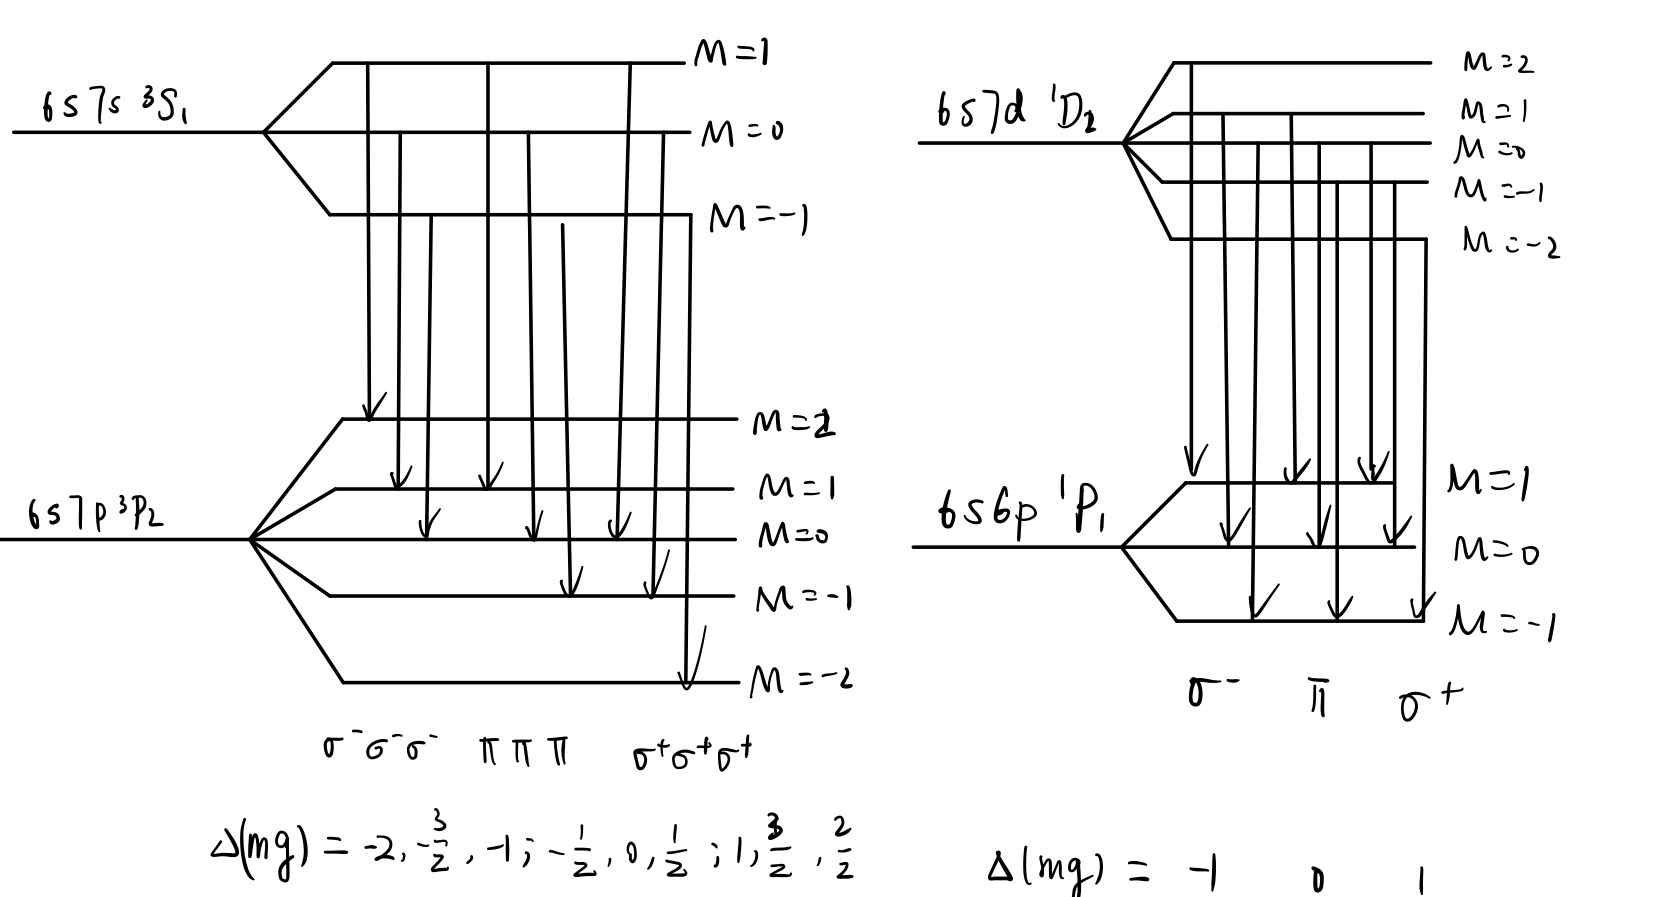
\includegraphics[width=\textwidth]{跃迁图.jpg}
\caption{汞绿线(左)和汞黄线(右)的塞曼效应跃迁情况}
\end{figure}

从上图中可以直观的看出, 外加磁场时, 汞绿线有9条分裂谱线, 汞黄线有三条分裂谱线. 
\section{实验}
本实验中使用的仪器是法布里珀罗标准具\cite{lecturenote}\cite{lecture}. 

标准具通过产生平行的多条光束, 通过会聚透镜在焦平面上发生干涉, 干涉处有
\begin{equation}
2d\cos{\theta}=K\lambda
\end{equation}
其中K为整数, 称之为干涉序. 容易知道, 干涉图样具有$\theta$相等的性质, 在平面上呈现圆环. 

本实验中, 在不加外磁场时, 谱线不会分裂, 因此需要关注波长固定$\lambda$的干涉特征; 在加入外磁场时, 由于原先干涉序为K的干涉环会分裂为多个环, 需要关注相同序下不同波长的干涉特征. 

下面引入$\theta<<1$的近似, 有
\begin{equation}
\cos{\theta}=1-\frac{D^2}{8f^2}
\end{equation}

其中f是透镜的焦距, D是$\theta$对应干涉环的直径, 而D恰好是本实验中主要的观测量. 

固定波长$\lambda$时, 我们会观察到圆环之间的直径差相等, 即
\begin{equation}
    \Delta D^{2}=D_{K-1}^{2}-D_{K}^{2}=\frac{4 f^{2} \lambda}{d}
\end{equation}

这一间隔与干涉序无关. 

考虑同一序的不同波长时, 注意到小角近似条件下, 圆环集中于中央, 干涉序通常很大, 可取$K\approx \frac{2d}{\lambda}$, 
此时有
\begin{equation}
    \lambda_{a}-\lambda_{b}=\frac{d}{4 f^{2} K}\left(D_{b}^{2}-D_{a}^{2}\right)=\frac{\lambda}{K} \frac{D_{b}^{2}-D_{a}^{2}}{D_{K-1}{ }^{2}-D_{K}{ }^{2}}
    =\frac{\lambda^{2}}{2 d} \frac{D_{b}^{2}-D_{a}^{2}}{{D_{K-1}}^{2}-D_{K}^{2}}
\end{equation}

以上式子用波数$\widetilde{\nu}=1/\lambda$表示将更加简洁: 
\begin{equation}
    \widetilde{v}_{a}-\widetilde{v}_{b}=\frac{1}{2 d} \frac{D_{b}^{2}-D_{a}^{2}}{{D_{K-1}}^{2}-D_{K}^{2}}=\frac{1}{2 d} \frac{\Delta D_{a b}{ }^{2}}{\Delta D^{2}}
\end{equation}

结合公式(5), 得到:
\begin{equation}
    \frac{e}{m}=\frac{1}{B d\left(\left(g_{1}-g_{2}\right) M_{1}-g_{2}\left(M_{2}-M_{1}\right)\right)} \frac{\left(D_{b}^{2}-D_{a}^{2}\right)}{\left(D_{K-1}^{2}-D_{K}^{2}\right)}
\end{equation}
此外, 我们还需要考虑分辨能力的问题. 一般而言, 法布里珀罗干涉仪生成的干涉环是极为尖锐的, 而不同波长的光束, 能有互不相干的一系列圆环干涉图样. 
在两种情况下, 干涉环之间将难以区分. 第一种是$\lambda_1$的干涉序$K$的圆环与$\lambda_2$的干涉序$K-1$的圆环重合时, 有
\begin{equation}
\Delta \lambda=\lambda_{2}-\lambda_{1}=\frac{\lambda^{2}}{2 d}
\end{equation}
这就是波长为$\lambda$的光束的极限分辨能力$\Delta \lambda$. 如果用波数表示, 结果将更为简洁: 
\begin{equation}
\Delta \tilde{v}=\frac{1}{2 d}
\end{equation}
这一结果只与标准具的参数有关, 称之为自由光谱范围. 

另一种情况下, 相同干涉序下波长差$\lambda_{a}-\lambda_{b}$极小而难以区分. 这里需要引入精细度的概念, 其定义是相邻条纹间距与条纹半宽度之比, 
经过计算发现它只与标准具的反射率R有关系: 
\be{F=\frac{\pi \sqrt{R}}{1-R}}

结合公式(5), (6), (11), 容易发现某一级谱线在磁场的作用下分裂时, 磁场越大, 分裂的程度越大, 越接近于自由光谱范围; 磁场越小, 分裂程度越小, 越接近于精细度. 
可见, 自由光谱范围和精细度确定了待观察的塞曼效应的磁场的上下限. 而自由光谱范围和精细度完全由标准具的参数d和反射率R所确定, 与具体的波长或者干涉序没有关系. 
\section{结果分析与讨论}
\subsection{标准具的自由光谱区计算以及磁场的上下限估计}
实验中使用的标准具$d=2mm$, 则自由光谱范围
\be{\widetilde{\nu}_{free}=\frac{1}{2d}=2.5 cm^{-1}}
在磁场$B=1T$时, 汞绿线的塞曼效应分裂间距为
\be{\widetilde{\nu}_{green}=\widetilde{L}/2=0.2335B=0.2335 cm^{-1}}
因此该磁场下自由光谱范围比汞绿线的分裂间距要大. 

当磁场大到一定程度时, 汞绿线干涉序K的外侧圆会与干涉序K-1的内侧圆相接触, 此时
\be{\widetilde{\nu}_{out}-\widetilde{\nu}_{in}=4\widetilde{L}=\widetilde{\nu}_{free} \Rightarrow B_{max}=1.338T}
我们一并对汞黄线的情况做相同的计算:
\be{\widetilde{\nu}_{out}-\widetilde{\nu}_{in}=2\widetilde{L}=\widetilde{\nu}_{free} \Rightarrow B_{max}=2.677T}

我们也尝试对能清晰观察到谱线分裂的磁场下界进行估计, 在临界情况时, 在公式(11)中, 粗略地认为$D_{k-1}+D_{K}\approx D_{a}+D_{b}$, $F^{-1}\approx(D_{a}-D_b)/(D_{k-1}-D_{K})$
\be{\widetilde{v}_{a}-\widetilde{v}_{b}=\frac{1}{2d}F^{-1}=\frac{1}{2d}\frac{1-R}{\pi \sqrt{R}}}
其中粗略取R=0.95. 

汞绿线的情形中, 公式左边取其塞曼谱线波数差$\widetilde{L}/2$, 有$B_{min}=0.175T$. 

汞黄线的情形中, 公式左边取其塞曼谱线中最大的波数差$\widetilde{L}$, 有$B_{min}=0.087T$. 

\subsection{B-I曲线的标定}
将霍尔特斯拉计调整至线圈中合适的位置, 开启电流, 调整电流输出的电压和电阻, 待特斯拉计读数稳定下来后进行记录. 电流上升阶段和下降阶段各测量一次。在测量开始时,发现特斯拉计无法调零,因此使用零点数据补偿有:$B_0=\SI{-73}{mT}$,矫正数据:$B = B_{measure} - B_0$
\bfig{0.9}{BI曲线.png}{BI曲线标定. 其中横轴为电流, 纵轴为磁场}

图例中的up表示电流依次增大时磁场测量的结果, down表示电流依次减小时磁场测量的结果. 可以看出, 相同电流下, 下降阶段的磁场略大于上升阶段的磁场, 
这符合我们对磁滞回线的预计. 相同电流处磁场在上升和下降阶段的偏差的量级在10mT, 相比于大尺度的变化(1000mT)而言很小, 因此可以说电流变化的历史不影响B-I曲线. 

为了后续根据电流标定磁场, 先分别将上升阶段和下降阶段的B-I曲线做多项式拟合. 这里拟合的工具采用的是mathematica中的NonLinearModelFit函数. 
由于两条曲线相差不大, 使用两个拟合公式的平均: 
\be{\overline{B}(I)=\frac{1}{2}(B_{up}(I)+B_{down}(I))=13.22 + 280.60 x + 26.10 x^2 - 6.55 x^3}
其中电流单位为A, 磁场的单位为mT.
\subsection{汞绿线的塞曼效应}
\subsubsection{磁场为零时的自由光谱}
本节意在验证公式(9), 即$\Delta{D}^2=D_{K-1}^2-D_{K}^2=\frac{4f^2\lambda}{d}$中, $\Delta{D}^2$与干涉序无关. 

对于汞绿线, 测量的情况如下图所示: 
\bfig{0.6}{free_g_measure.png}{无外加磁场时的汞绿线谱线}
由于此处是单张图片, 为了便于打印, 对图片做了颜色负片(即黑白反转). 此时黑色的线即表示干涉环, 绿线(红线的负片)表示测量时作的圆. 
图中测量了四个圆的半径, 分别为K级圆, K-1级圆, K-2级圆, K-3级圆的半径, 测量和计算的结果如下: 

\begin{table}[H]
    \centering
    \begin{tabular}{|c|c|c|}
    \hline
    干涉序    & D      & $D_{k-1}^2-D_K^2$  \\ \hline
    K   & 265.25 &          \\ \hline
    K-1 & 387.07 & 79465.62 \\ \hline
    K-2 & 480.99 & 81538.20 \\ \hline
    K-3 & 559.38 & 81550.60 \\ \hline
    \end{tabular}
    \caption{汞绿线的无磁场光谱测量. (单位: pix(像素))}
    \end{table}
$\Delta D^2$的偏差大概为$2000pix^2$, 相对偏差为$2000/80000\approx 2.5\%$, 可见$\Delta D^2$的确是不随干涉序变化的. 

\subsubsection{加磁场后谱线的分裂情况}
从零开始逐渐增大电流, 会观察到谱线逐渐变粗, 逐渐分裂扩张. 对于汞绿线的情形, 有三个阶段值得关注: (1)分裂初见端倪(2)谱线的分裂比较明显(3)谱线中K级最外侧圆与K-1级最内侧圆接触, 达到自由光谱极限. 
这三个阶段分别如下所示: 

\begin{figure}[H]
    \centering
    \begin{subfigure}[b]{0.3\textwidth}
      \centering
      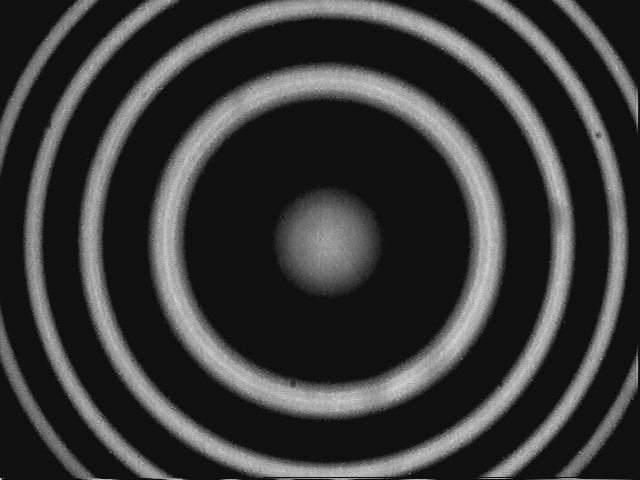
\includegraphics[width=\textwidth]{MultiRings@1.5A.jpg}
      \caption{分裂初见端倪, 此时I=1.5A}
    \end{subfigure}
    \hfill
    \begin{subfigure}[b]{0.3\textwidth}
      \centering
      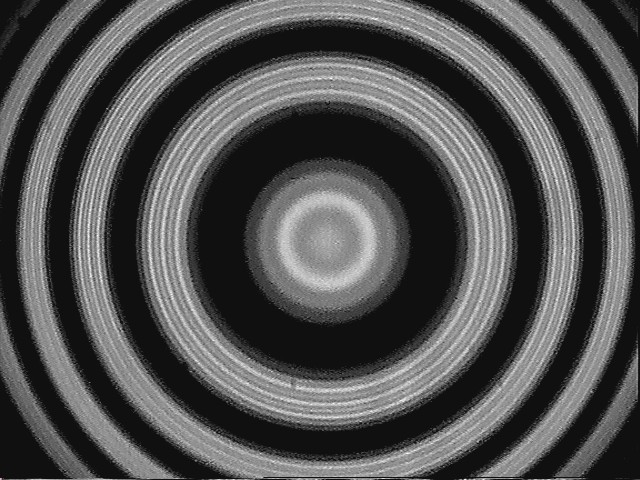
\includegraphics[width=\textwidth]{MultiRings@2.52A.jpg}
      \caption{观察到明显分裂, 此时I=2.52A}
    \end{subfigure}
    \hfill
    \begin{subfigure}[b]{0.3\textwidth}
      \centering
      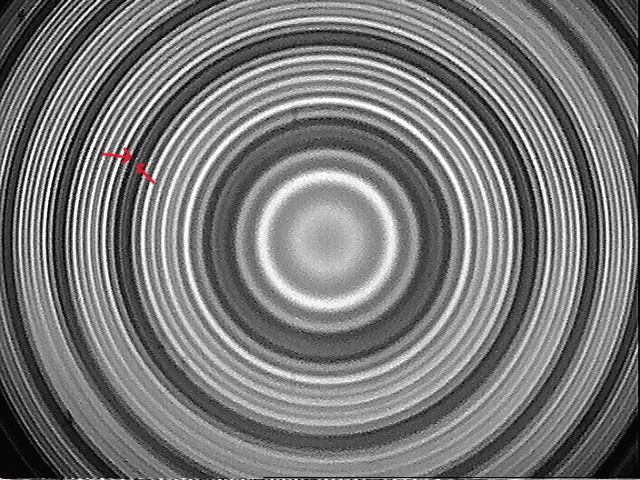
\includegraphics[width=\textwidth]{MultiRings@4.63A.jpg}
      \caption{分裂达到极限, 此时I=4.63A}
    \end{subfigure}
    \caption{汞绿线的谱线分裂情况}
  \end{figure}

在上图(c)中, 标记了内圈K级中心圆和外圈K-1级中心圆, 箭头所指处为重合K级最外侧圆与K-1级最内侧圆重合处. 由于此处是三张小图, 且(c)的条纹较密, 
取负片以后黑白条纹容易混淆, 故此处不取负片. 

根据前述B-I标定的结果(公式(21)), 汞绿线的这三种情况依次对应磁场0.471T, 0.781T, 1.222T. 前面理论上预计的最大电流$B_{max}$为1.338T, 与我们此处的测量接近, 
但理论上预计的$B_{min}=0.175T$, 对应于能够观察到清晰的谱线分裂的临界磁场, 却比测量结果(0.471T)要小许多, 原因除了前面估算时可能带来的误差以外, 还有实验中光路调节不佳, 使谱线不够细锐的原因. 

就实验本身的测量结果应为, 电流处于1.5A-4.63A时, 能够观察到汞绿线的塞曼效应分裂, 这对应的磁场为0.471T-1.222T. 

\subsubsection{塞曼效应的偏振效应}
实验在垂直磁场方向对汞绿线的塞曼效应谱进行观察, 理论上预计会观察到9条分裂谱线, 其中中间3条是偏振方向平行于磁场的$\pi$线, 左右两边的6条是偏振方向垂直于磁场的$\sigma$线. 
在旋转偏振片的过程中, 会观察到$\pi$线和$\sigma$线的依次消光. 

下图呈现了旋转偏振片过程中实验观测的结果, 左中右分别是9条谱线, 6条谱线, 3条谱线的结果. 

\begin{figure}[H]
    \centering
    \begin{subfigure}[b]{0.3\textwidth}
      \centering
      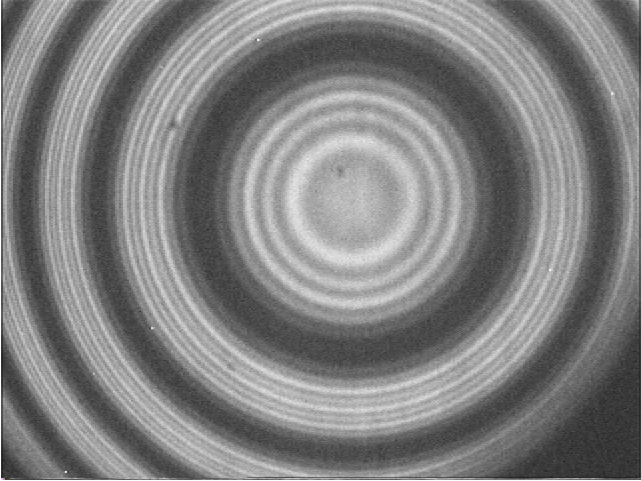
\includegraphics[width=\textwidth]{2.74gp.jpg}
      \caption{透过偏振片, 观察到9条谱线}
    \end{subfigure}
    \hfill
    \begin{subfigure}[b]{0.3\textwidth}
      \centering
      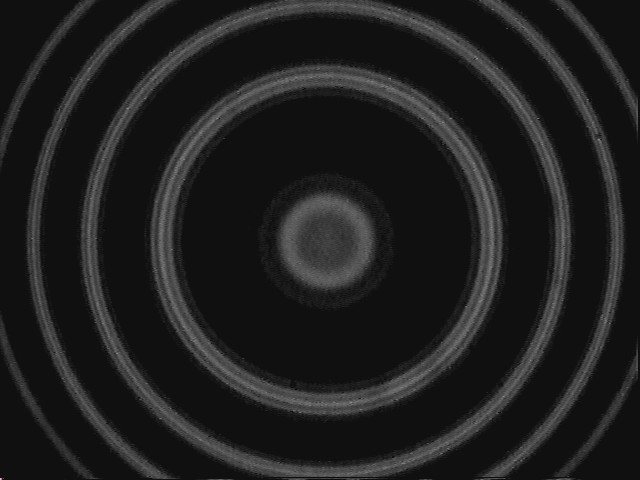
\includegraphics[width=\textwidth]{MultiRings-polorizeB.jpg}
      \caption{透过偏振片, 观察到6条谱线}
    \end{subfigure}
    \hfill
    \begin{subfigure}[b]{0.3\textwidth}
      \centering
      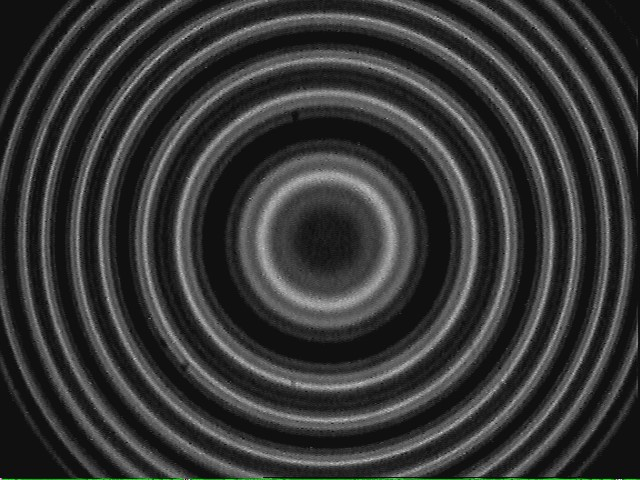
\includegraphics[width=\textwidth]{MultiRings-polorizeA.jpg}
      \caption{透过偏振片, 观察到3条谱线}
    \end{subfigure}
    \caption{汞绿线的塞曼效应谱的偏振情况}
  \end{figure}

上图中图(b)呈现了3条$\pi$线, 对应于$\sigma$线的消光, 对应于偏振片的透振方向平行于磁场. 注意到图(b)中还有一些隐约的$\sigma$线, 这些线在实验中
能够通过降低亮度消除, 但无法通过旋转偏振片消除. 可能的原因是, 在这个方向上圆, 偏振光$\sigma$线本应呈现线偏振, 但由于实验中的光路没有完全垂直于磁场, 以致于呈现的是椭圆偏振光, 在平行
于磁场方向上仍能观测到$\sigma$分量. 

上图中图(c)呈现了6条$\sigma$线, 对应于$\pi$线的消光, 对应于偏振片的透振方向垂直于磁场. 由于$\pi$线本身就是线偏振光, 在垂直于磁场的方向上消除的很好, 没有残留的分量. 

由于光路调节的不佳, 在偏振角处于一定范围内的情况下, 偏振情况大致不变. 图(b)对应的偏振角是$302°-321°$, 该区间的中心为$311.5°$; 图(c)对应的偏振角是$35°-59°$, 该区间的中心为$47°$. 可见区间之间大致相差90°, 
符合我们理论的预计, 但由于光路调节不佳, 仍有一定偏差. 

\subsubsection{从谱线间距反推磁场}
在通过偏振片消去谱线内外的$\sigma$线后, 剩余的三条$\sigma$线很难超过自由光谱极限. 故在使用偏振片消去$\sigma$线后, 利用$\pi$线的谱线间距进行测量. 
此时每一级只有三个圆. 对于某个电流值, 分别测量K级中心圆, K-1级中心圆和内外两侧的圆的直径. 
实验中选取了6个电流值进行测量, 结果如下表: 
\begin{table}[H]
    \centering
    \begin{tabular}{|c|c|c|c|c|c|c|}
    \hline
    I(A)&3A&3.5A&4A&4.5A\\ \hline
    第K级中心圆&336.40&338.20&336.36&338.43\\ \hline
    第K级外侧圆&353.58&353.19&354.78&361.44\\ \hline
    第K-1级外侧圆&492.63&492.84&494.37&495.30\\ \hline
    \end{tabular}
    \caption{选取不同电流, 谱线干涉环的直径测量. 直径的单位: pix(像素)}
    \end{table}


实验中所测量的内外侧圆之间, 彼此之间的波数间隔为$\widetilde{L}/2$. 利用公式(11), 可以分别推算外侧线与中心线, 中心线与内侧线的波数差. 通过对两个波数差取平均, 可以推算该电流下的洛伦兹单位$\widetilde{L}$, 
从而推知磁场. 
使用的公式可以整理为: 
\be{B=\frac{1}{0.467}\frac{\left |D_{K-1_{out}}^2-D_{K-1_{mid}}^2\right | + \left |D_{K_{out}}^2-D_{K_{mid}}^2\right |}{2d\left |D_{K-1_{mid}}^2-D_{K_{mid}}^2\right|}}

其中$D_{K_{mid}}$, $D_{K-1_{mid}}$, $D_{K_{out}}$, $D_{K-1_{out}}$分别对应K级中心圆, K-1级中心圆和K级外侧圆, K-1级外侧圆的直径.

计算的结果, 以及用拟合公式(21)在相应电流处拟合的结果一并放在下表中: 
\begin{table}[H]
    \centering
    \begin{tabular}{|c|c|c|c|c|c|}
    \hline
    I&3.00A&3.50A&4.00A&4.50A\\ \hline
    $B_{measure}$ & 0.96 & 1.10 & 1.23 & 1.48 \\ \hline
    $B_{fit}$     & 0.91 &1.03 & 1.13 & 1.20\\ \hline
    $r$ & 6.0\%	&7.0\%	&9.0\% &	23\%\\ \hline

    \end{tabular}
    \caption{通过谱线反推的磁场与拟合的电流比较值. $B_{measure}$是用公式(22)计算的结果, $B_{fit}$是用公式(21)计算的结果. $r$是相对误差, 定义为$r=\left | B_{fit}-B_{measure}\right |/B_{fit}$}
    \end{table}

    实验测量的结果除去在$\SI{4.50}{A}$下测量的结果,其他结果相对于B-I标定曲线的偏差在10\%以内, 为了更直观地看到其中的差距, 将实验测量的结果与B-I标定曲线放在一起, 如下图所示: 
    \bfig{0.6}{B_measure.png}{实验测量结果与B-I标定曲线对比}
该实验结果与前面拟合得到的结果相差较大,且有偏大的系统误差。对此我们做一下解释:
\begin{itemize}
  \item 在测量圆环半径时,由于使用了手动标定法,手动标定相邻内外侧环时,由于为了清晰分辨,可能会有人为的将两圆环分得较开的倾向,这导致了实验测量的结果相对于拟合结果偏大。
  \item 在测量电流为$\SI{4.5}{A}$的数据时,可以看到绘制外侧圆环有较大的偏外趋势,这导致了$\SI{4.5}{A}$数据有较大的偏差。
  \bfig{0.3}{MultiRings@4.50A_measure.jpg}{4.5A下的圆环测量}
  \item 在实验中,由于光路调节不佳,导致了谱线不够细锐,这也会导致实验测量的结果相对于拟合结果偏大。
  \item 实验中还存在一种固有误差, 来自于霍尔磁力计的放置的位置, 与汞光源的位置不一定一致, 也会带来一定的误差。
  \item 此外霍尔磁力计也只能测量一个方向上的磁场, 也会带来一定的误差。
  \item 测量时,测量使用的CCD像素大小也会带来误差,这一部分误差的估计在后文中给出。
\end{itemize}
这里我们讨论一下CCD带来的误差:先假设标定干涉环的直径时有1个像素大小的不确定度(由于圆心的定位以及取点带来的不确定度). 该不确定度的合理性可以从表2中K级中心圆半径和K-1级中心圆半径的变化中看出, 这两个
干涉环与零磁场的谱线重合, 理论上不应随磁场变化, 但实际上仍然有一定偏差. 这意味着公式(22)中所有的直径都有$u(D)=1$. 在此基础上, 将不确定度公式
\be{ u(W)=\sqrt{\sum_{i=1}^{N}\left(u\left(x_{i}\right) \frac{\partial W}{\partial x_{i}}\right)^{2}}}
作用于公式(22)时, 以电流$I=4A$的数据为例, 将有
\be{u(B)=0.0565T \Rightarrow r(B)=\frac{u(B)}{B}=4.12\%}
因此可以在表3中看到, 实验测量带来的误差没有太偏离估计.  

\subsection{汞黄线的塞曼效应}
\subsubsection{磁场为零时的自由光谱}
在光路不进行调整的情况下, 依次测量无磁场下汞绿线的光谱和汞黄线的光谱, 如下图所示: 
\begin{figure}[H]
    \centering
    \begin{subfigure}[b]{0.45\textwidth}
      \centering
      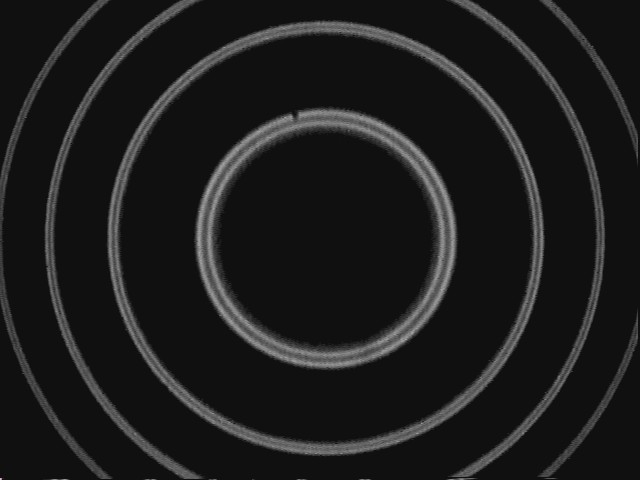
\includegraphics[width=\textwidth]{Doublerings.jpg}
      \caption{汞绿线自由光谱}
    \end{subfigure}
    \hfill
    \begin{subfigure}[b]{0.45\textwidth}
      \centering
      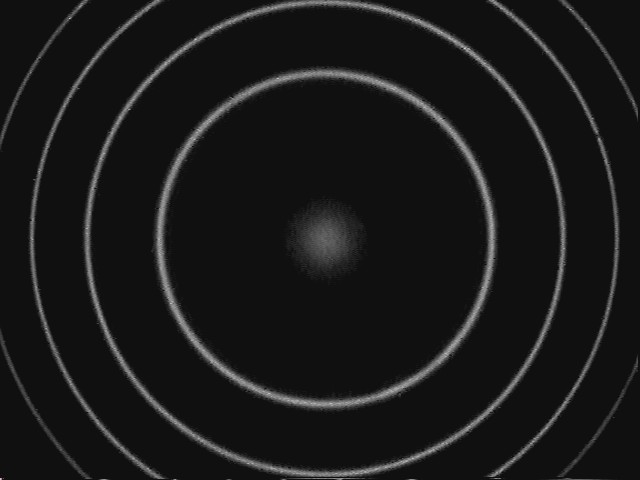
\includegraphics[width=\textwidth]{SingleringCompare.jpg}
      \caption{汞黄线自由光谱}
    \end{subfigure}
  \caption{无磁场情况下汞绿线和汞黄线的光谱}
  \end{figure}
  汞绿线和汞黄线的光谱存在细微差异。为了进一步说明这一点,我们可以通过数值方法生成干涉圆,即给定波长$\lambda$后,绘制一系列干涉圆。
  生成干涉圆时,需要确定圆的级次和直径。同时,为了提高计算的准确性,我们在公式(7)中不再做小角近似,而是采用以下表达式:
\be{\cos{\theta}=\frac{f}{\sqrt{D^2/4+f^2}}}
将此代入公式(7)后,可以求得干涉圆直径$D(\lambda,K)$为:
\be{D(\lambda,K)=2f \sqrt{\frac{4d^2}{K^2\lambda^2}-1}}
在阐释圆与圆之间的大小关系时可以将前面的系数2f略去. 
接下来是确定要画的圆的级次. 中心处应有$K=2d/\lambda$. 同时我们简单考虑空气的折射率n=1.00027, 则汞绿线(真空波长546.074nm)有K=7323.04, 汞黄线(真空波长576.959nm, 以及579.065nm)有K=6931.03, 6905.82. 
则对汞绿线来说, 作干涉序7323-7319的圆, 汞黄线中波长较大的作干涉序6931-6927的圆, 波长较小的作干涉序6905-6901的圆, 将有下面的图\cite{塞曼效应实验中法布里-珀罗标准具的Matlab模拟}\cite{塞曼效应实验报告}: 
\begin{figure}[H]
    \centering
    \begin{subfigure}[b]{0.32\textwidth}
      \centering
      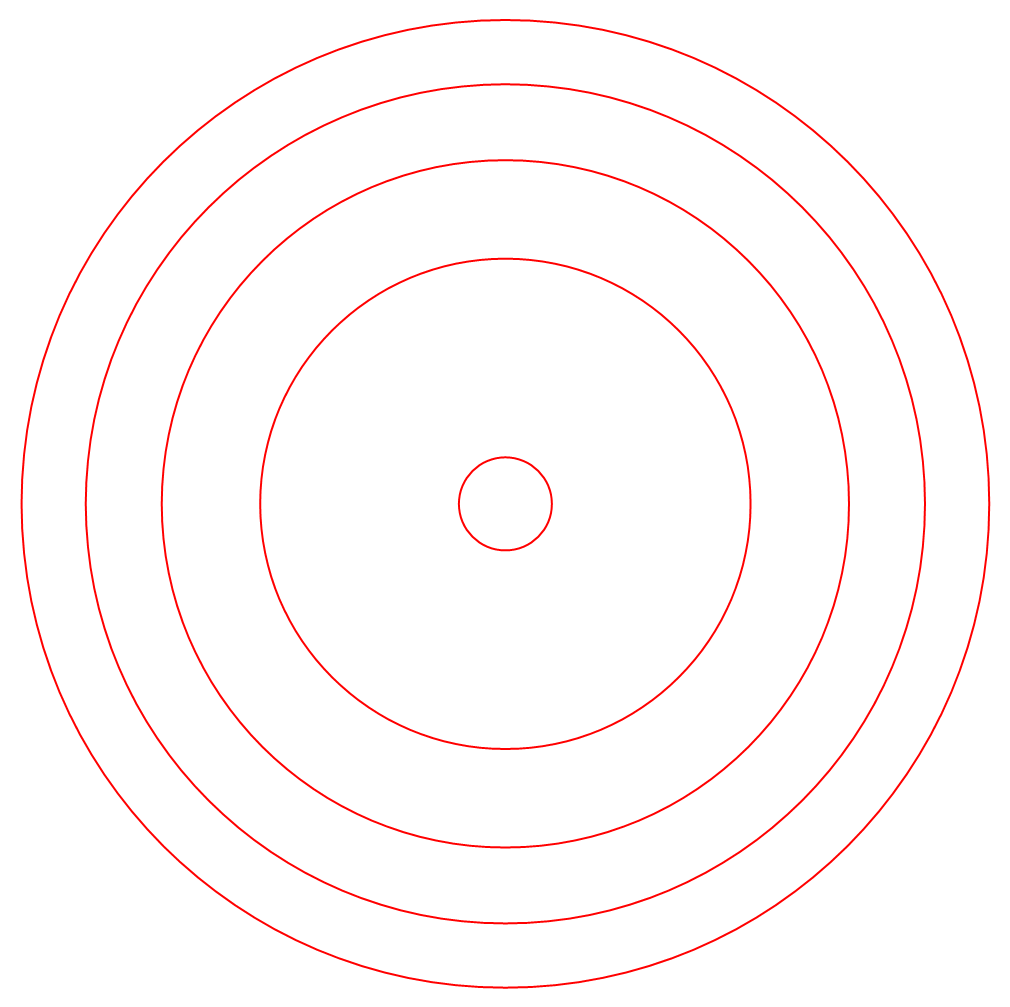
\includegraphics[width=\textwidth]{calc_g}
      \caption{汞绿线干涉环示意图}
    \end{subfigure}
    \hfill
    \begin{subfigure}[b]{0.32\textwidth}
      \centering
      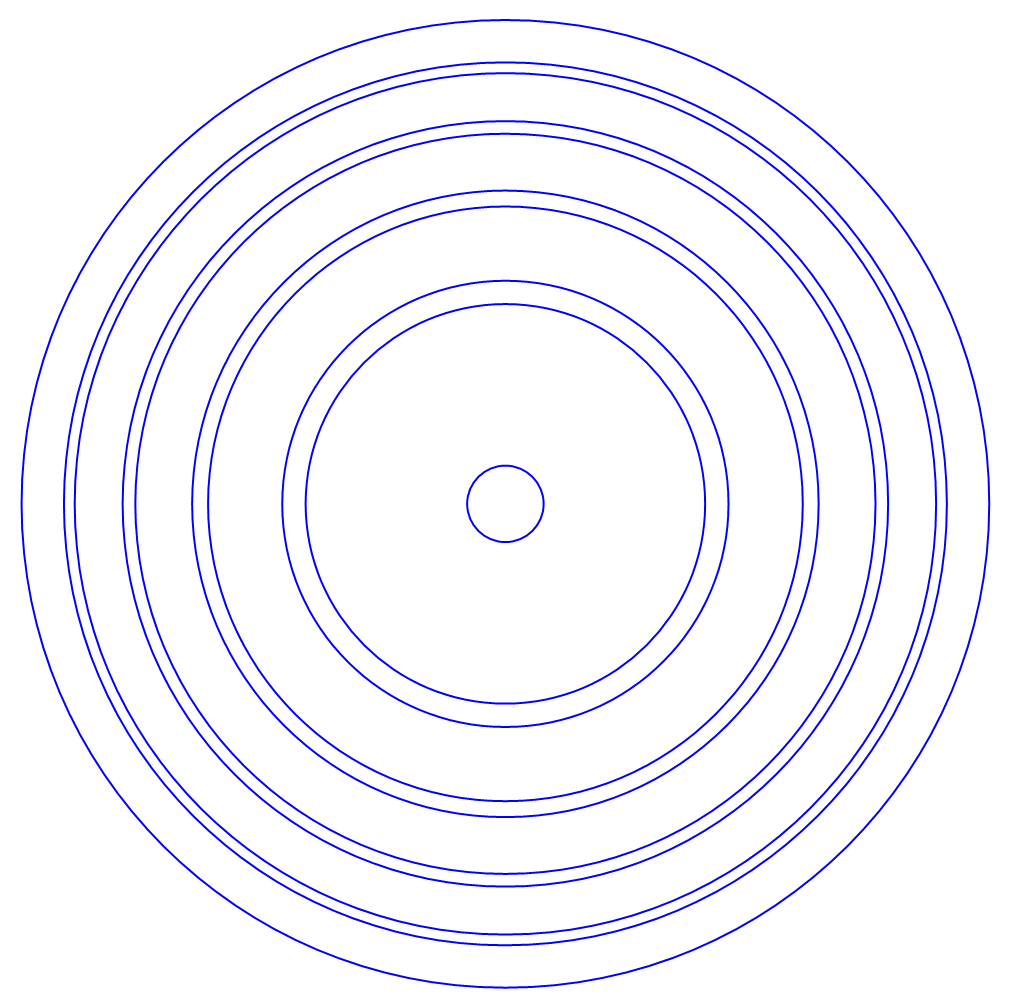
\includegraphics[width=\textwidth]{calc_y}
      \caption{汞黄线双线示意图}
    \end{subfigure}
    \hfill
    \begin{subfigure}[b]{0.32\textwidth}
      \centering
      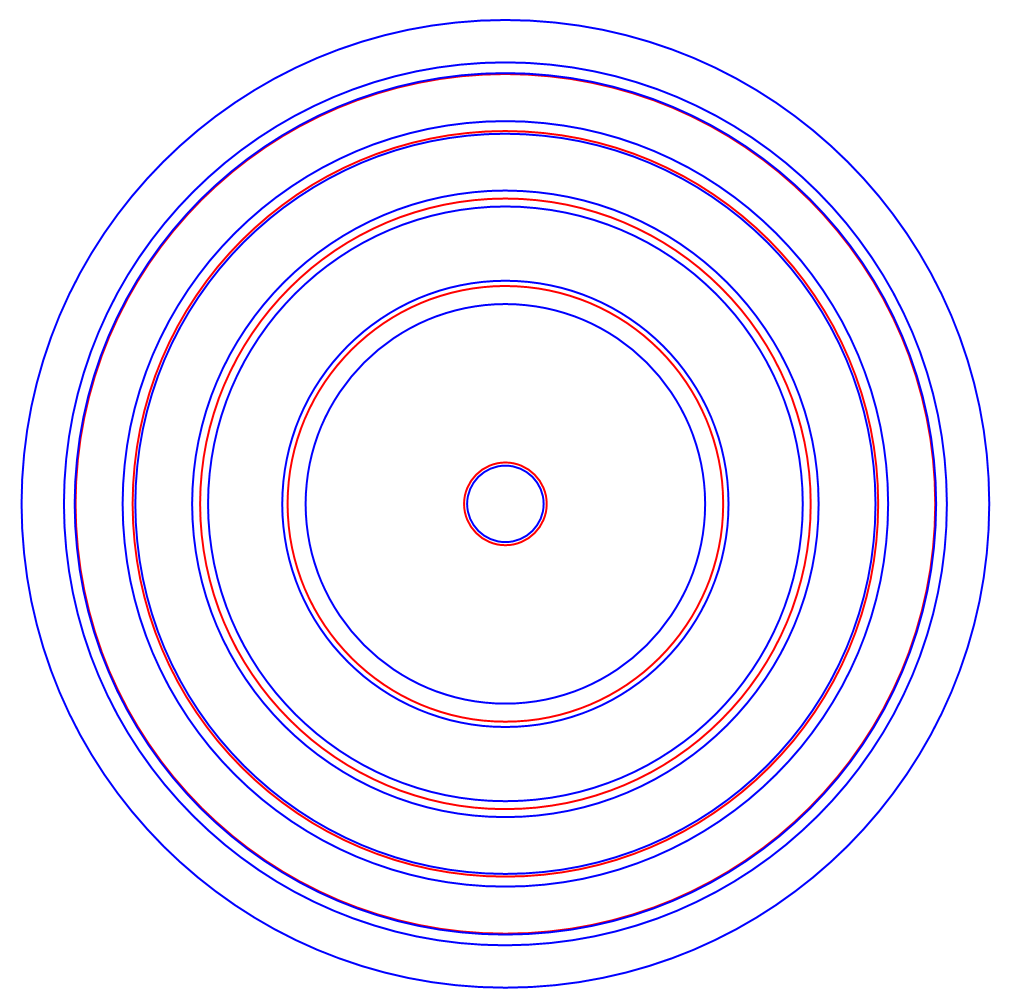
\includegraphics[width=\textwidth]{calc_yg}
      \caption{将两图合在一起}
    \end{subfigure}
    \caption{汞绿线和汞黄线的干涉环计算结果}
  \end{figure}
从图中可以看出两个重要信息: (1)汞黄线的双线其实相距很近, 并且随着半径的增大越来越接近. 但需要注意的是这两条线的级次其实相去甚远. (2)在光路不改变的情况下, 汞绿线和汞黄线的位置大致重合. 
因此在图7(b)中心看到的双峰确实就是汞黄线的双线, 往外的第一条线能隐约分辨, 再往外就由于光路不佳, 无法分辨了. 

另外需要指出, 作图的结果很大程度上取决于中心的$K=2d/\lambda$的下界整数影响, 这很受选取的真空波长的参考值和空气折射率影响, 所做的图仅有示意作用. 

\subsubsection{加磁场后谱线的分裂情况}
从零开始逐渐增大电流, 会观察到谱线逐渐变粗, 逐渐分裂扩张. 对于汞绿线的情
形, 有三个阶段值得关注: (1) 分裂开始能被观测到 (2) 谱线的分裂比较明显 (3) 谱线中 K 级
最外侧圆与 K-1 级最内侧圆接触, 达到自由光谱极限. 这三个阶段分别如下所示:
\begin{figure}[H]
    \centering
    \begin{subfigure}[b]{0.3\textwidth}
      \centering
      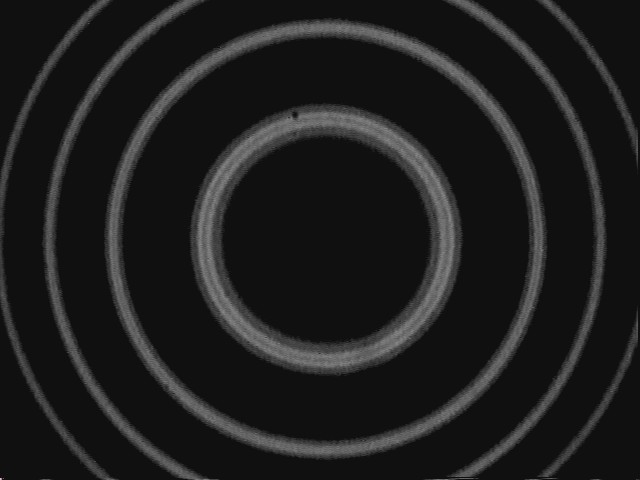
\includegraphics[width=\textwidth]{Multirings@0.90A.jpg}
      \caption{分裂开始能被观测到, 此时I=0.90A}
    \end{subfigure}
    \hfill
    \begin{subfigure}[b]{0.3\textwidth}
      \centering
      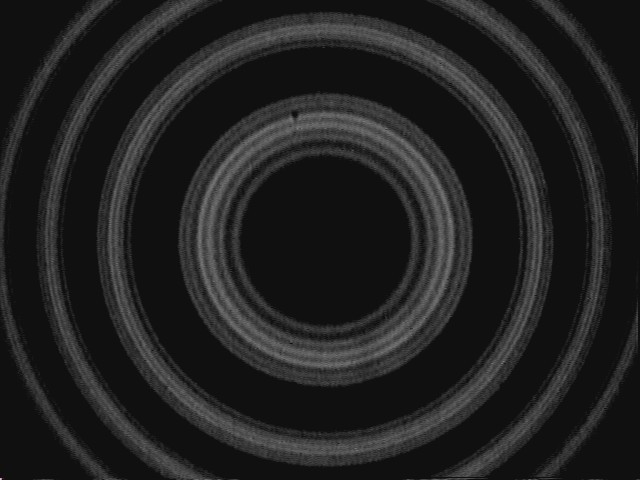
\includegraphics[width=\textwidth]{Multirings@2.55A.jpg}
      \caption{观察到明显分裂, 此时I=2.55A}
    \end{subfigure}
    \hfill
    \begin{subfigure}[b]{0.3\textwidth}
      \centering
      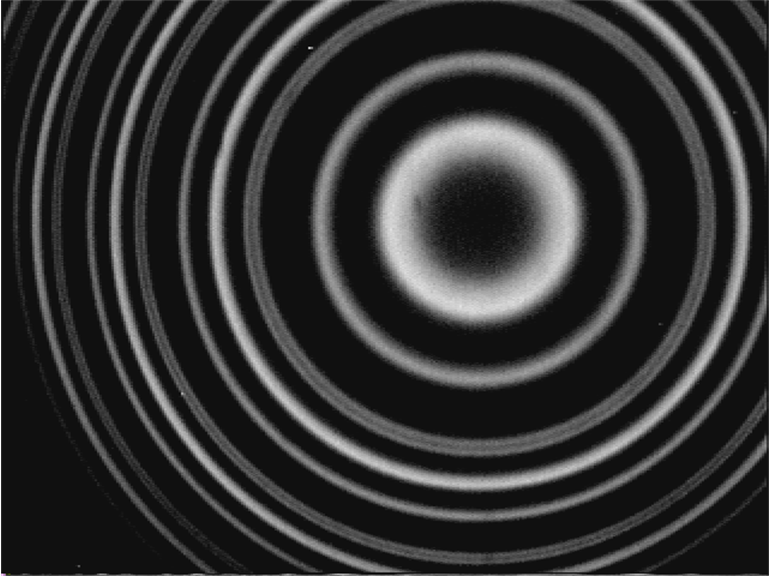
\includegraphics[width=\textwidth]{4.68yy.png}
      \caption{电流调至最大, 此时I=5.05A}
    \end{subfigure}
    \caption{汞黄线的谱线分裂情况}
  \end{figure}
  根据前述 B-I 标定的结果 (公式 (21)), 汞黄线的这三种情况依次对应磁场 0.28T,
  0.79T, 1.25T. 前面理论上预计的最大电流 Bmax 为 2.677T, 实验中调不出这么大的磁场, 因此观察不到自由光谱极限. 
  理论上预计的 Bmin = 0.087T, 对应于能够观察到清晰的谱线分裂的临界磁场, 却比
  测量结果 (0.28T) 要小许多, 原因除了前面估算时可能带来的误差以外, 还有实验中光
  路调节不佳, 使谱线不够细锐的原因. 
  
  关于这一点, 还有另一个值得一提的原因. 汞黄线的双线结构来自于$6{ }^{3} \mathrm{D}_{2}-6{ }^{1} \mathrm{P}_{1}$, 和$6{ }^{1} \mathrm{D}_{2}-6{ }^{1} \mathrm{P}_{1}$, 
  前者对应于反常塞曼效应, 与中心波长的波数差依次为8/6,7/6,1,1/6,0,-1/6,-1,-7/6,-8/6. 后者对应于正常塞曼效应, 波数差为-1,0,1. 可以看到, 汞黄线的反常塞曼效应应有9条谱线, 其中每3个一组, 都在其正常塞曼效应的三条谱线附近, 混在一起无法分开, 
  因此通常情况下只能观察到3条分裂谱线. 
  
\subsubsection{塞曼效应的偏振效应}
实验在垂直磁场方向对汞黄线的塞曼效应谱进行观察, 理论上预计会观察到 3 条分
裂谱线, 其中中间 1 条是偏振方向平行于磁场的 $\pi$ 线, 左右两边的两条是偏振方向垂直
于磁场的 $\sigma$ 线. 在旋转偏振片的过程中, 会观察到 $\pi$ 线和 $\sigma$ 线的依次消光.
下图呈现了旋转偏振片过程中实验观测的结果, 左右分别是 2 条谱线, 1 条谱线的结果.
\begin{figure}[H]
    \centering
    \begin{subfigure}[b]{0.45\textwidth}
      \centering
      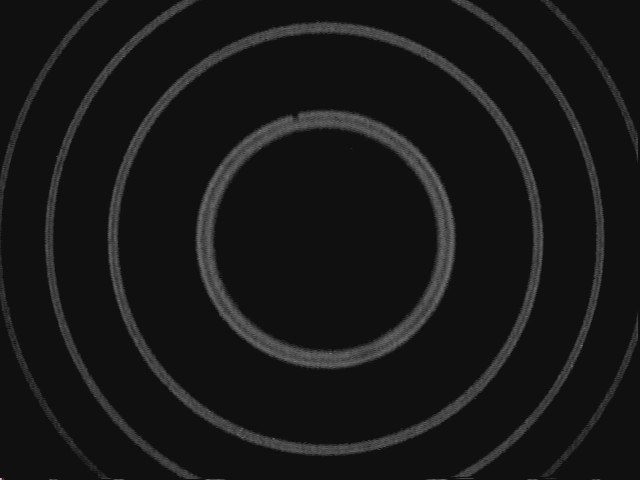
\includegraphics[width=\textwidth]{Multirings@2.55A_polorizedA.jpg}
      \caption{汞黄线的偏振: 2条}
    \end{subfigure}
    \hfill
    \begin{subfigure}[b]{0.45\textwidth}
      \centering
      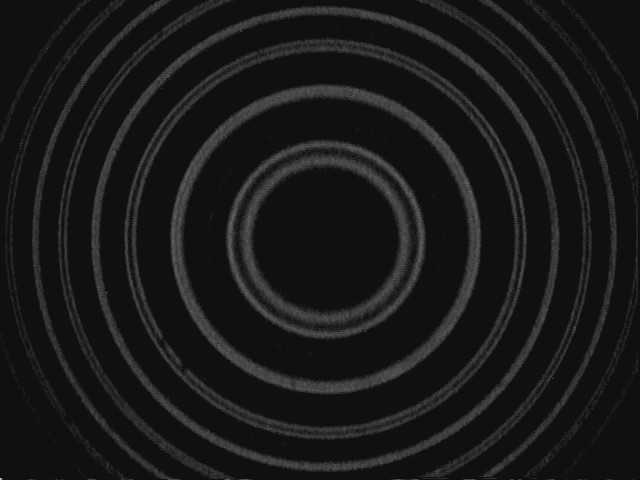
\includegraphics[width=\textwidth]{Multirings@2.55A_polorizedB.jpg}
      \caption{汞黄线的偏振: 1条}
    \end{subfigure}
  \caption{汞黄线塞曼效应的偏振现象}
  \end{figure}
可以看到, 在这种情况下, 汞黄线的双线结构更加明显. 

上图中图 (a) 呈现了 2 条 $\sigma$ 线, 对应于 $\pi$ 线的消光, 对应于偏振片的透振方向垂直于磁场. 

上图中图 (b) 呈现了 1 条 $\pi$ 线, 对应于 $\sigma$ 线的消光, 对应于偏振片的透振方向平行
于磁场. 

由于光路调节的不佳, 在偏振角处于一定范围内的情况下, 偏振情况大致不变. 图
(a) 对应的偏振角是 43°-51.5°, 该区间的中心为 47.25°; 图 (b) 对应的偏振角是 304°−320°,
该区间的中心为 312°. 可见区间之间大致相差 90°, 符合我们理论的预计, 但由于光路
调节不佳, 仍有一定偏差.此结果与上面测量汞绿线的偏振效应的结果是不一致,检查偏振片发现:偏振片相对固定夹具有松动,旋转和调整过程中发生偏移,导致了实验结果的不一致。这也可能是导致测得偏振不完全垂直的原因之一。
\subsection{平行磁场方向的塞曼效应}
\subsubsection{平行磁场方向观察汞绿线的塞曼效应}
调整光源方向,透过546nm滤色片观察汞绿线的塞曼效应,此时磁场方向与光路方向平行。在此情况下,观察到的谱线如下图所示:
首先是无磁场下的谱线:
\begin{figure}[H]
    \centering
    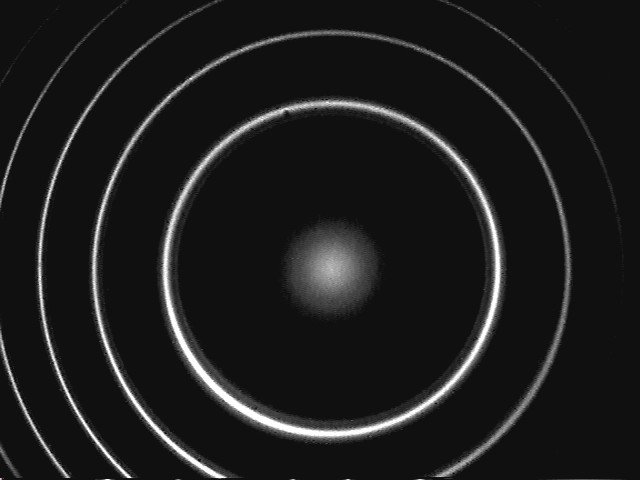
\includegraphics[width=0.5\textwidth]{SingleRingh.jpg}
    \caption{无磁场下的汞绿线谱线}
\end{figure}
可以看到,此时观察到的是单线结构,与垂直磁场方向获得的谱线几乎无差异。接下来是加磁场后的谱线:
\begin{figure}[H]
    \centering
    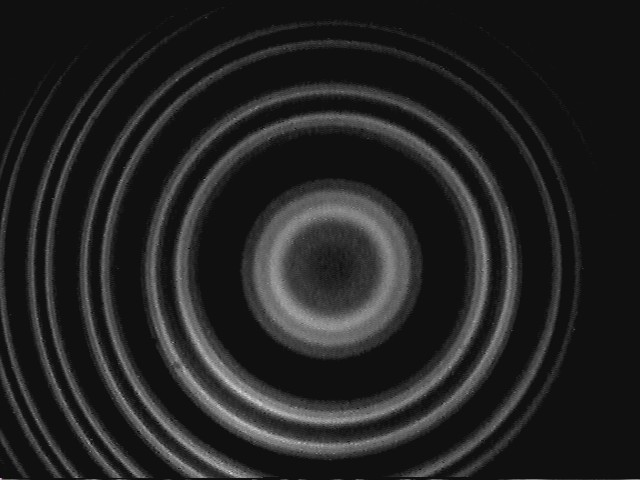
\includegraphics[width=0.5\textwidth]{MultiRing@2.50A.jpg}
    \caption{加磁场后的汞绿线谱线}
\end{figure}
观察此时的谱线,发现相较垂直磁场方向观察到的谱线,中央谱线谱线缺失,只留下正向和反向分裂的谱线,这是由于磁场方向与光路方向平行,导致$\pi$线的消失。这也是塞曼效应的一个重要特征。
\subsubsection{平行磁场方向汞绿线塞满分裂的偏振效应}
在平行磁场方向观察汞绿线的塞曼效应时,同样可以观察到偏振效应。在旋转偏振片的过程中,会观察到所有的谱线都变暗淡并且不随着旋转角度的变化而变化,这是由于磁场方向与光路方向平行,导致了$\pi$线的消失。这也是塞曼效应的一个重要特征。这说明留下的谱线如果有偏振态应当是圆偏振光。于是向偏振片前加入一个四分之一波片,将左旋圆偏振光和右旋圆偏振光转化为相互垂直的线偏振光。
然后转动偏振片,观察到的两组谱线的消失和出现如下图所示:
\begin{figure}[H]
    \centering
    \begin{subfigure}[b]{0.45\textwidth}
      \centering
      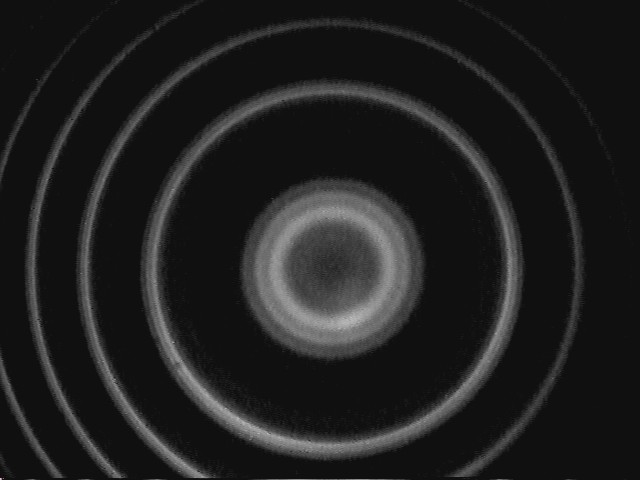
\includegraphics[width=\textwidth]{MultiRing@2.50A_CircularlPolorizedA.jpg}
      \caption{汞绿线的左旋偏振: 3条}
    \end{subfigure}
    \hfill
    \begin{subfigure}[b]{0.45\textwidth}
      \centering
      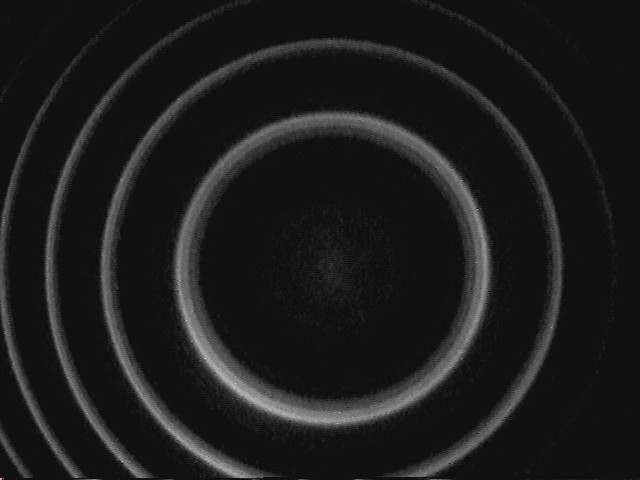
\includegraphics[width=\textwidth]{MultiRing@2.50A_CircularlPolorizedB.jpg}
      \caption{汞绿线的右旋偏振: 3条}
    \end{subfigure}
  \caption{汞绿线塞曼效应的偏振现象}
  \end{figure}
  可以看到,当偏振片的透振方向与圆偏振光的偏振方向平行时,观察到的谱线消失,当偏振片的透振方向与圆偏振光的偏振方向垂直时,观察到的谱线出现。这说明留下的谱线是圆偏振光。这也说明了塞曼效应的偏振效应。
\section{总结}
实验中使用F-P腔, 在垂直于磁场的方向上对汞绿线和汞黄线在光源处于不同磁场下的干涉环进行了观测. 在不外加磁场的情况下观察到了汞绿线的单线结构和汞黄线的双线结构, 使用数值计算对观测图样进行了确认. 在外加磁场的情况下观察到了汞绿线的反常塞曼效应, 汞黄线的正常塞曼效应. 使用偏振片, 在垂直于磁场的方向上观测到了
$\pi$线和$\sigma$线的消光, 消光时两者的偏振片方向正交. 利用汞绿线的$\pi$线在磁场下的劈裂, 测量了分裂谱线的直径, 反推了中心磁场的大小, 和事先标定的结果的差异在5\%上下, 并从不确定度和磁力计本身的问题的不同角度对此误差进行了分析. 
\printbibliography
\section{附录: 原始数据}
\begin{figure}[H]
    \centering
    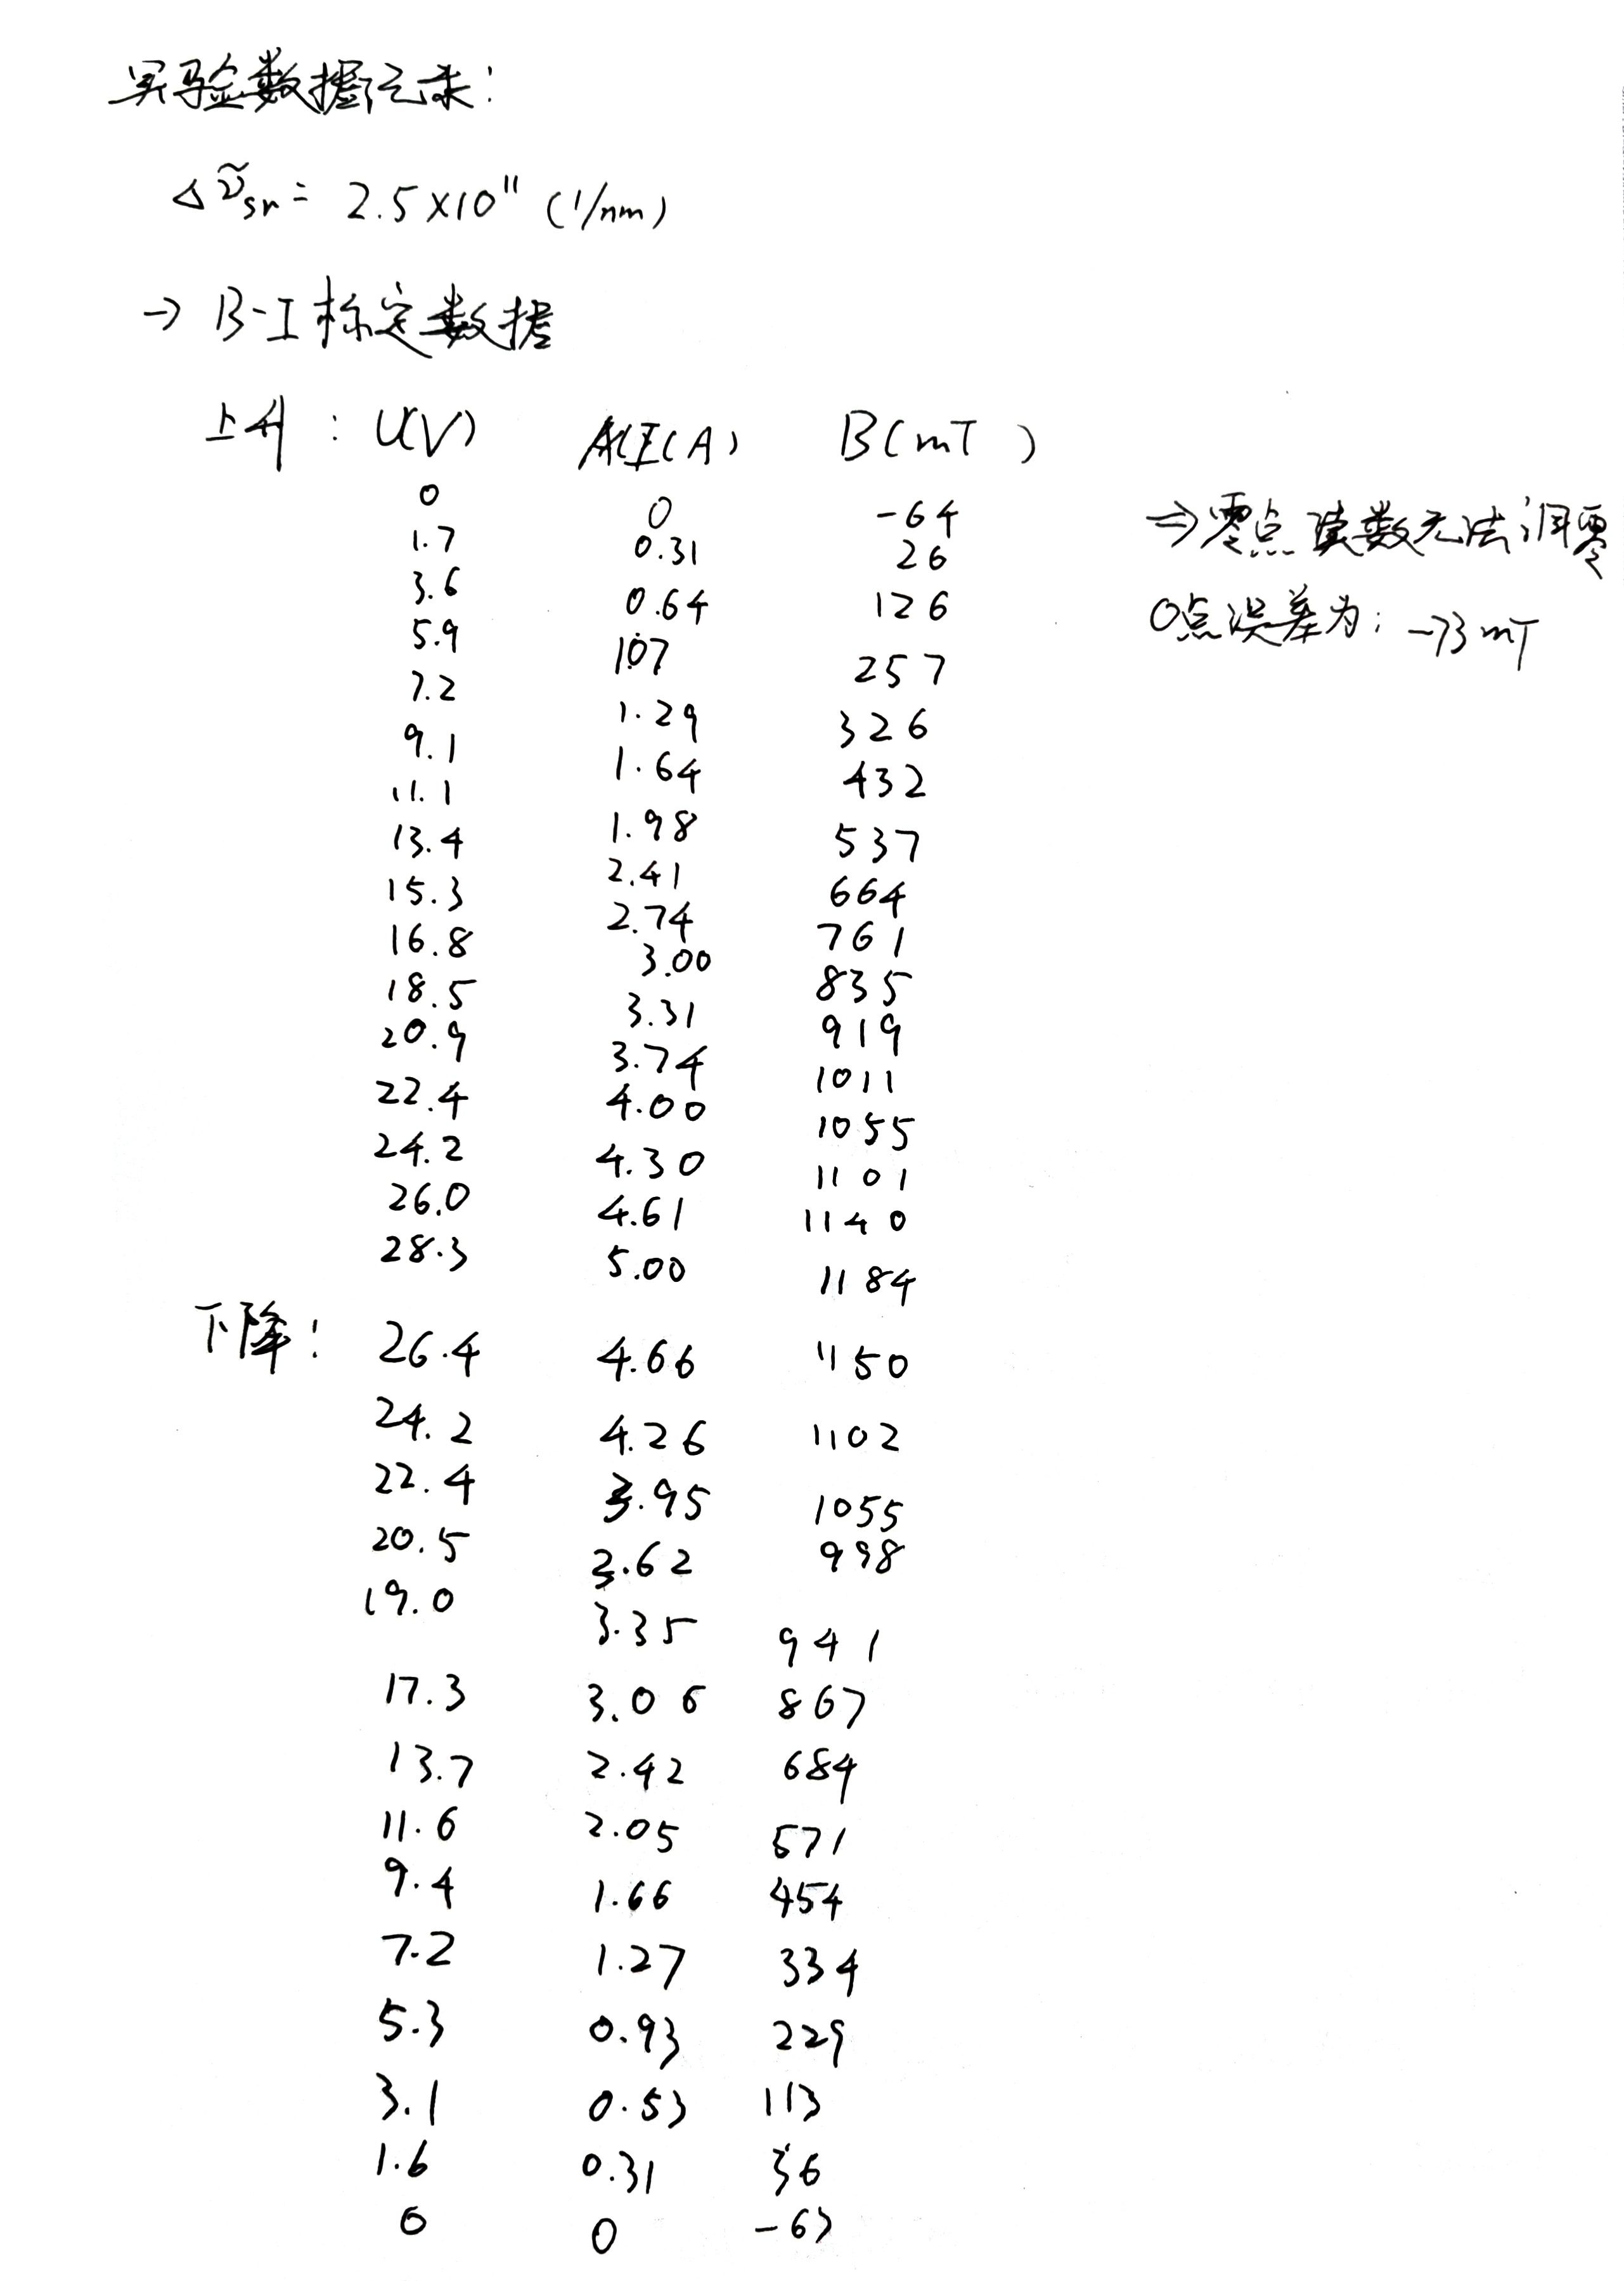
\includegraphics[width=0.5\textwidth]{Ata1.jpg}
    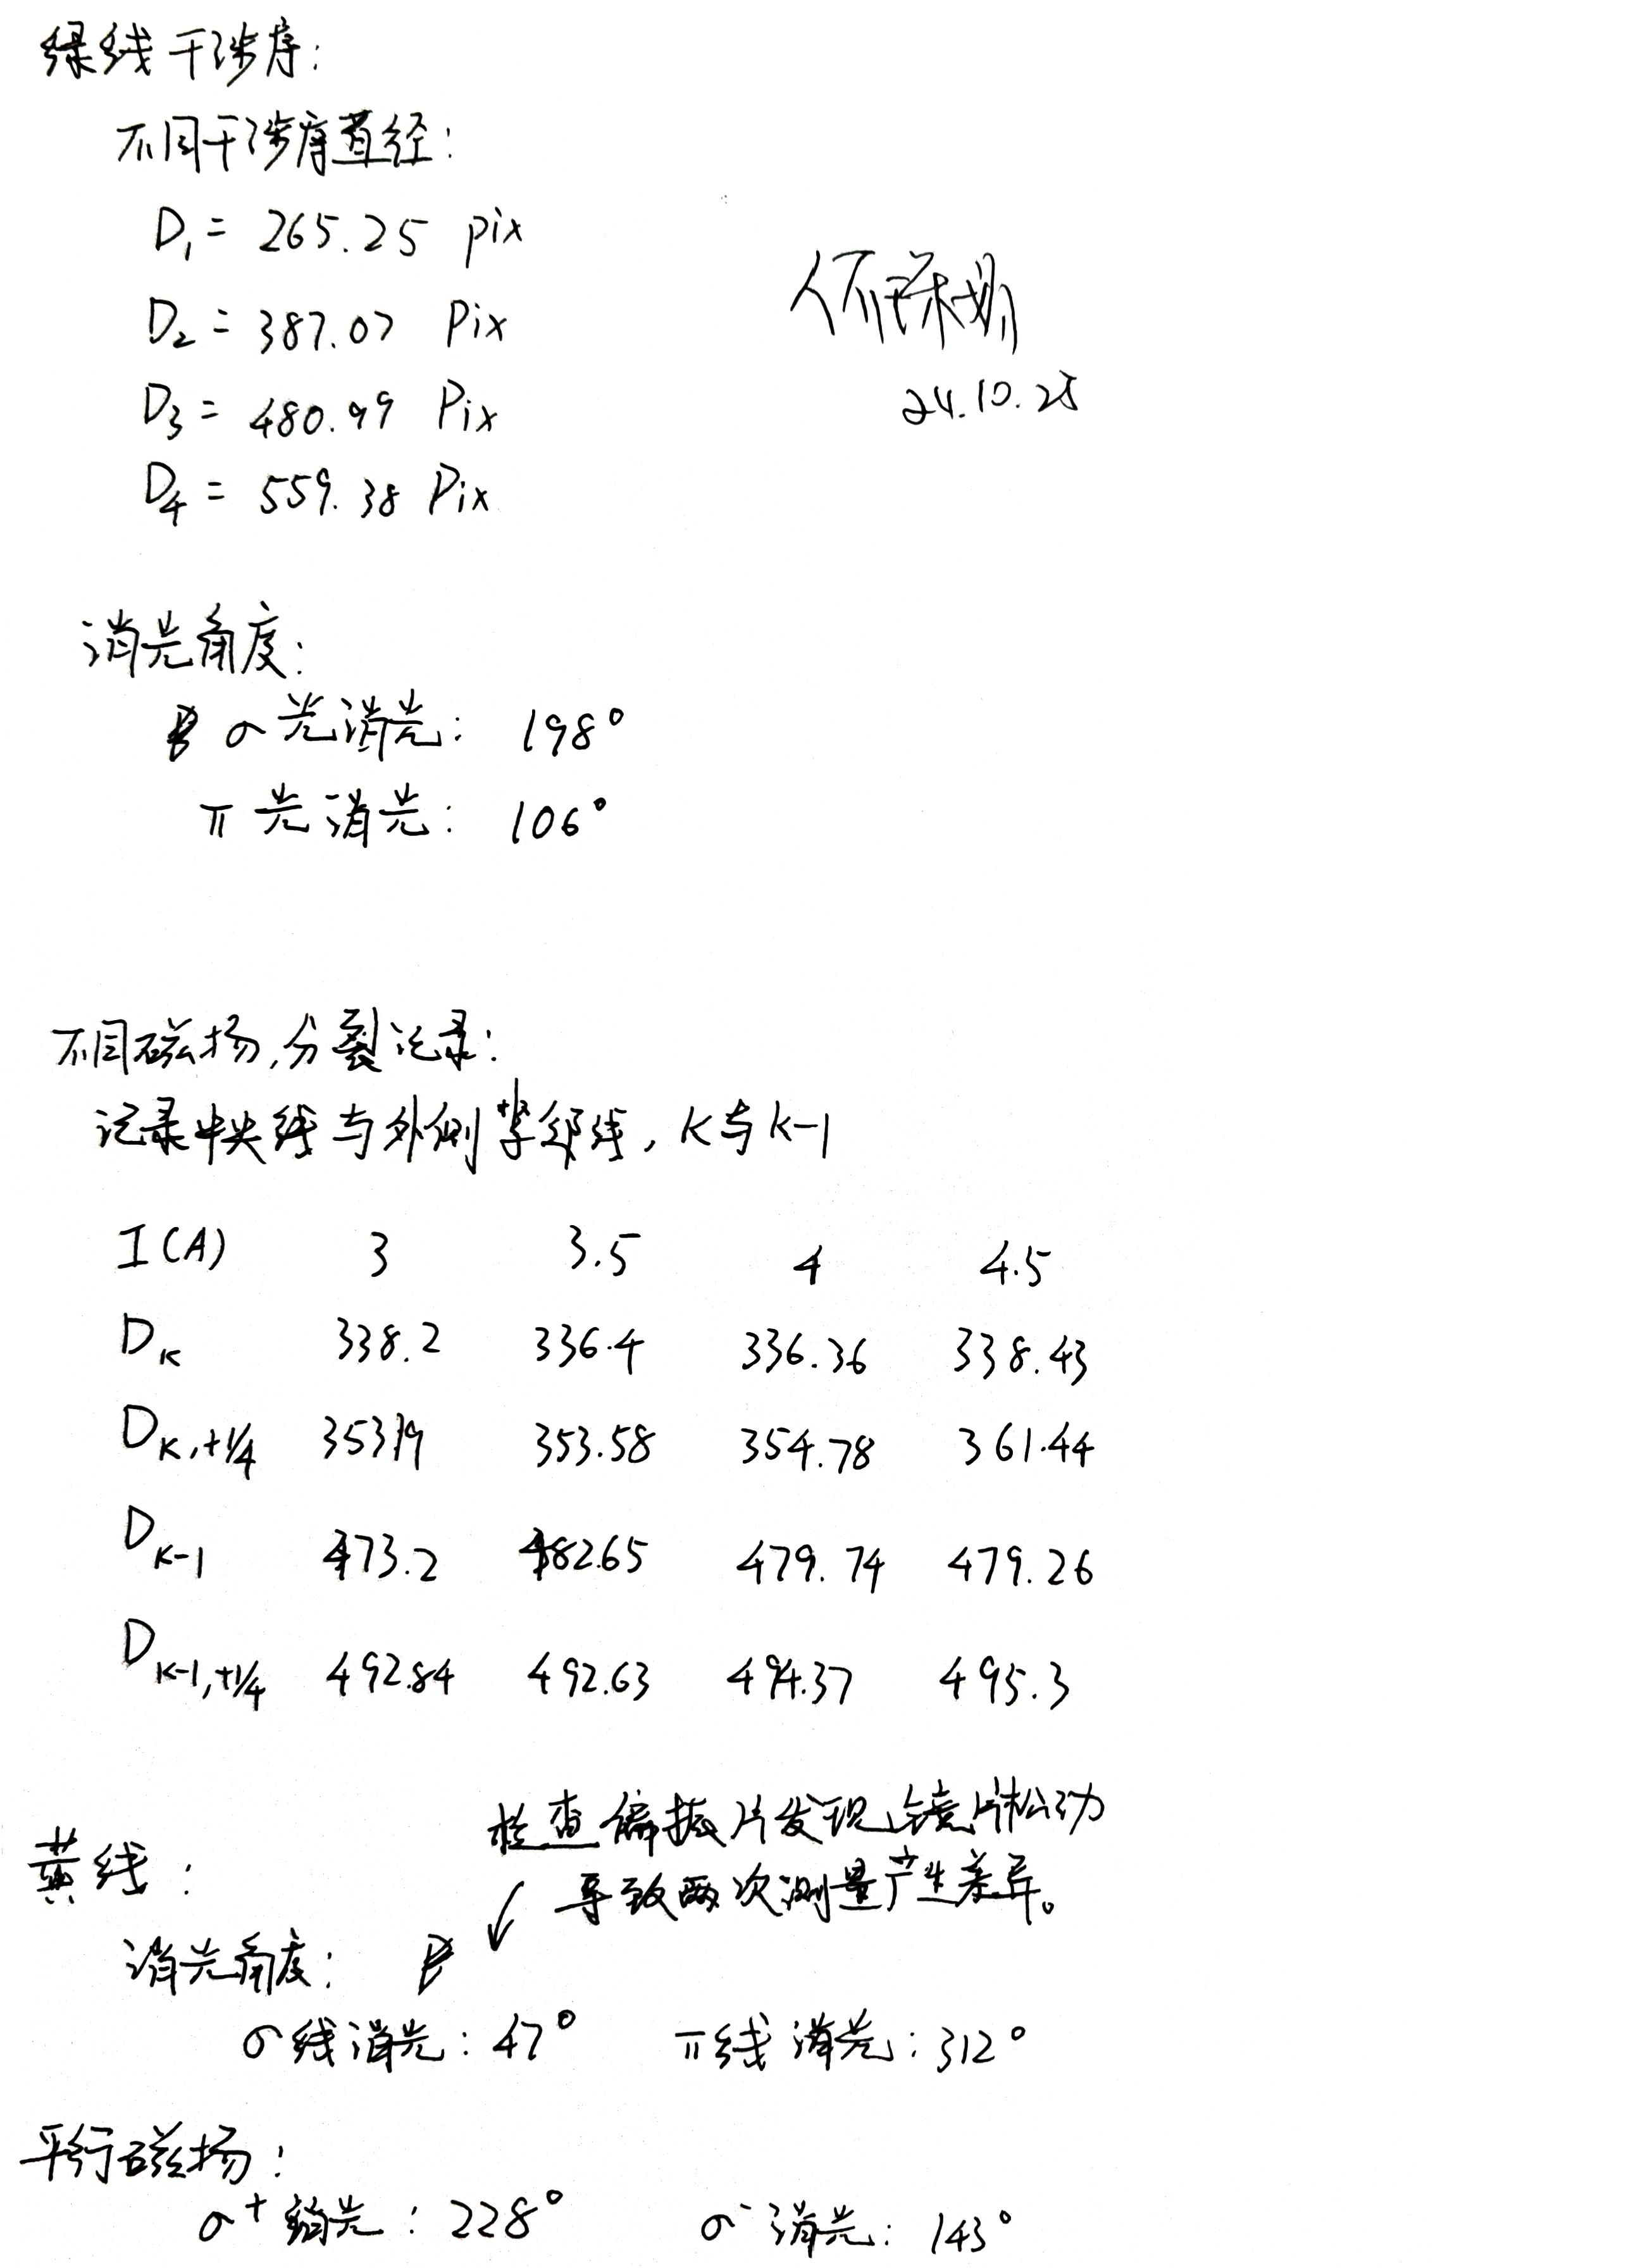
\includegraphics[width=0.5\textwidth]{Ata2.jpg}
\end{figure}


\end{document}